\chapter{Discussion}
	This chapter will summarize and discuss the results in the previous chapter.

\section{Guidance System}
	The guidacen system are greately simplifyed. In this section these simplifications will be adressed
	and other possible errors and shorcomings will be treated. 

	This Guidance system are designed for long, straight pipeline streches. It will not be able to handle
	sudden turns in the pipeline direction, without spcifying this in the guidance system. This can be
	included as waypoints where the pipeline are changing, and be included as a condition; \textit{when the AUV
	reaches certain position the direction of the pipeline changes}. This requiers very exact knowledge
	about the pipeline and are rearly the case. TThis is why there should be a more autonomous way of
	doing this. This motivates the use of more sensros than just a camera to follow the pipeline. The
	camera have a very limited field of view, usually restricted to less than 3 meters. A Side Scan Sonar
	comined wiht a Forward Looking Sonar, which provides sensor data of the pipeline in front of the AUV
	will give the guidance system some data to descide and predict what it will do if there is a sharp
	turn in the pipeline. 

	Sharp turns are rare, and are a product of T-junctions and other couplings of pipelines. These
	junctions are usually well documented, and given good and exact locations. But if the navigation
	sensors of the AUV have large uncertanties, and from the AUV it might look as they are in the wrong
	place. This suggests that information about the pipeline should be treated with care. Because the
	errors in an AUV navigation system might be substantial and provide that \'a priori information about
	the pipeline will be unusable. 

	The navigation system of \textit{HUGIN 1000} are a Velocity Aided Inertial Navigation System. This
	utilises a Doppler Velocity Log to measure the velocity relatively to the sea bottom and input this to
	the INS system. The INS systems usually installedn on the \textit{HUGIN} are in the 1 nmi/h class, i.e
	the INS system drifts less than 1 nmi/h. This results in a drift in the navigation system equal to
	0.11 \% of the traveled distance along the track, and about 0.03 \% error in the across distance of a
	stright line track. \cite{INS_Hugin}. This can be enough to throw the guidance system off course,
	because the field of view of the camera are relatively small.

	***********************************************

	There are ways of improving the INS drift, one is to use GPS update fixes, but this requiers to
	surface the AUV once in a while. This is of course not a good idea when the AUV are at great depths.
	There are posibilities to use sea bottom anchored position bouys, which exact position are known and
	the AUV might use these bouys by pinging them and getting a updated position estimate. This is a good
	idea if the pipeline infrastructure admints this. Say that this position bouys are placed at the same
	time as the pipeline are layed, but this is a costly affair. 

	Too use a Ultra Short Base Line (USBL) are another posibility. A USBL transducer are mounted on a
	ship, which has a GPS location fix. The AUV then pings the USBL transducer regularily and the position
	are determined exactly. This requiers a ship stationed in the area where the AUV are carrying out the
	mision. The autonomicity of the AUV are the reduced, and the vehicle are not capable of operating on
	its own. 

	**********************************************

	The problem regarding when $\psi \rightarrow 2\pi$ problem, there are a number of solutions for this.
	The first is to limit the sensor output, which are the case in the real world, since a compass
	measuring \textit{yaw} only are defined for $(0, 2 \pi)$. The controller can handle this by including
	a chech wheter if its heading are larger than $\pi$, the given command will be to the right, and
	opposite if the measured heading are smaller than $\pi$.

	\subsection{Increasing the inspection speed}
		What happens when the inspection speed are increased beyond 1 m/s? Say if the surge velocity
		were to be increased to 2 m/s. 




\section{Roll Stabilization}
	The mission of the AUV are to provide good data for later use, i.e good pictures to be analyzed later.
	The camera on the AUV are mounted downwards and the field of view are affected by roll and pitch.
	Pitch are a contorl angle, but the Roll motion have no direct control measures. The roll angle need to
	be as close to 0 as possible to provide best pictures of the current sea bottom. Imagine if the AUV
	were to move upside-down above the sea bottom. The plots in Figure~\ref{fig:ch4_rollyawmoment}
	are taken from the $4^{\mathrm{th}}$ Scenario described in Chapter~\ref{ch3}, to look at \textit{HUGIN
	1000}'s stability in roll.
	
	\begin{figure}[htbp]
		\centering
		\subfigure[Roll Angle]{
			\label{fig:ch4_rollangle}
			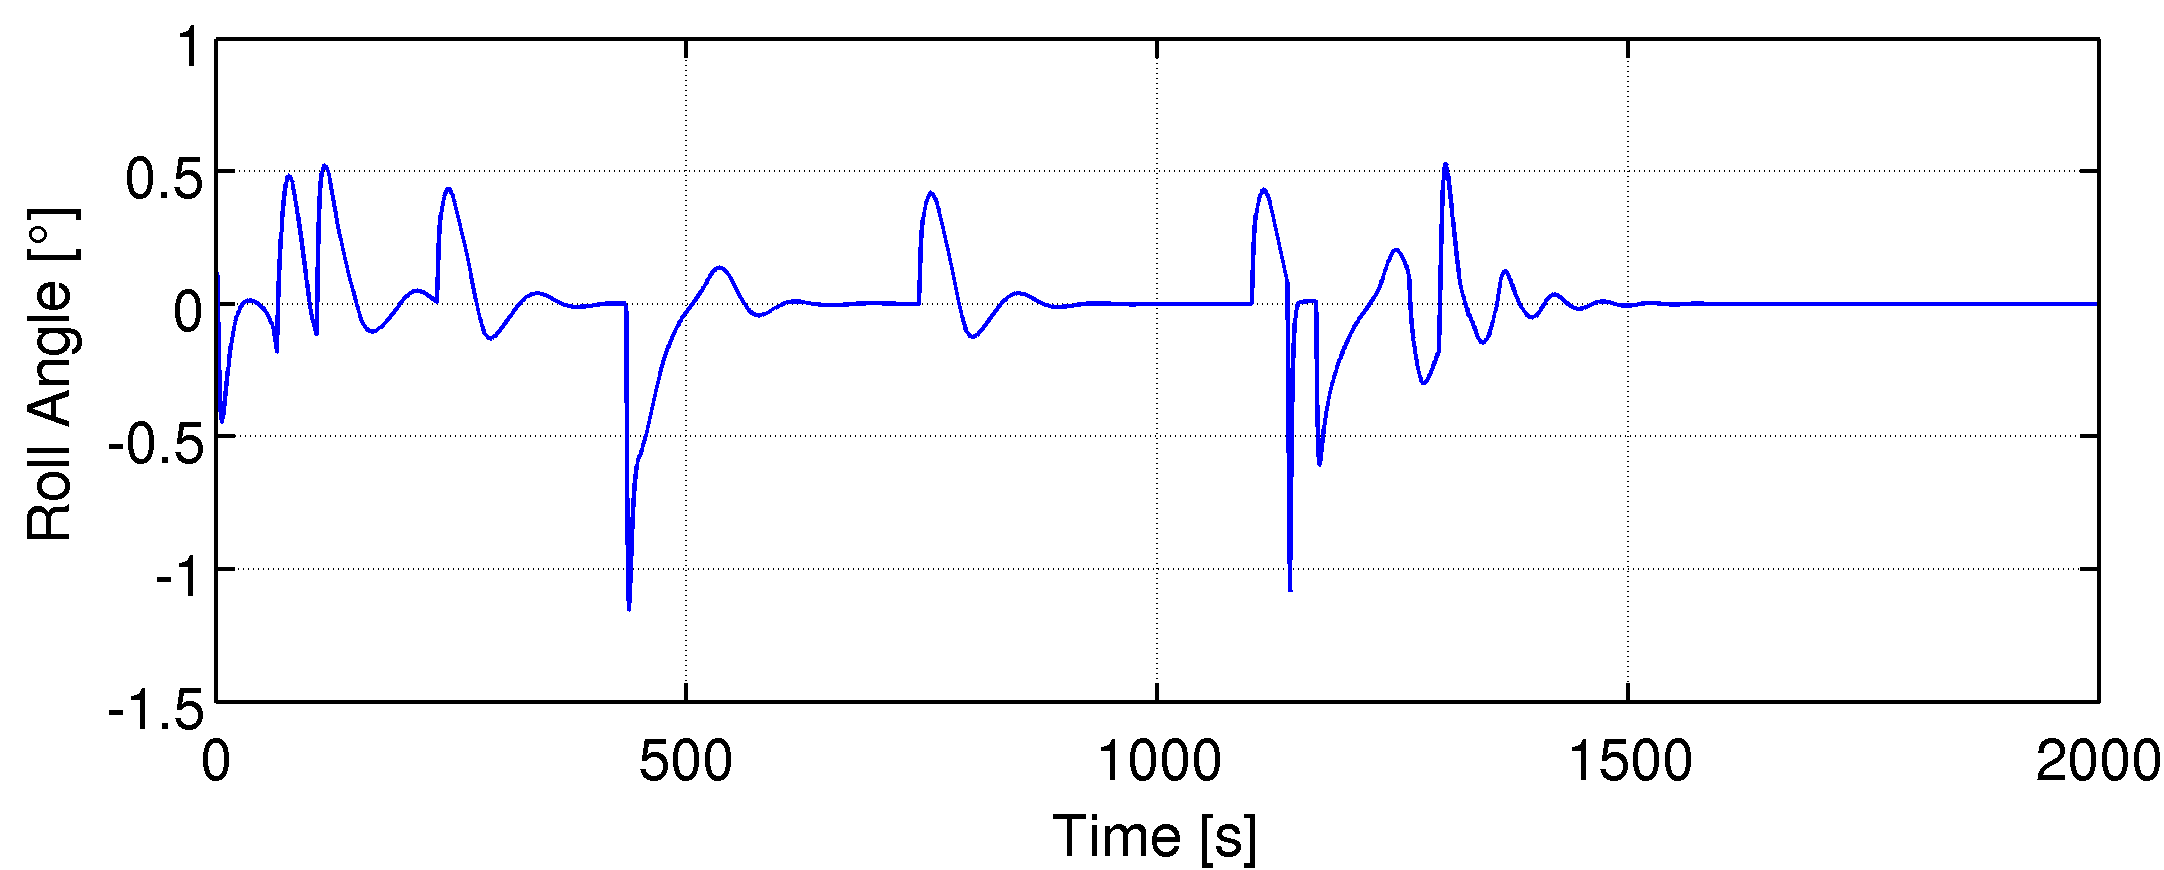
\includegraphics[width=0.7\textwidth]{pics/ch4_rollangle}}
		\subfigure[Yaw Moment]{
			\label{fig:ch4_yawmoment}
			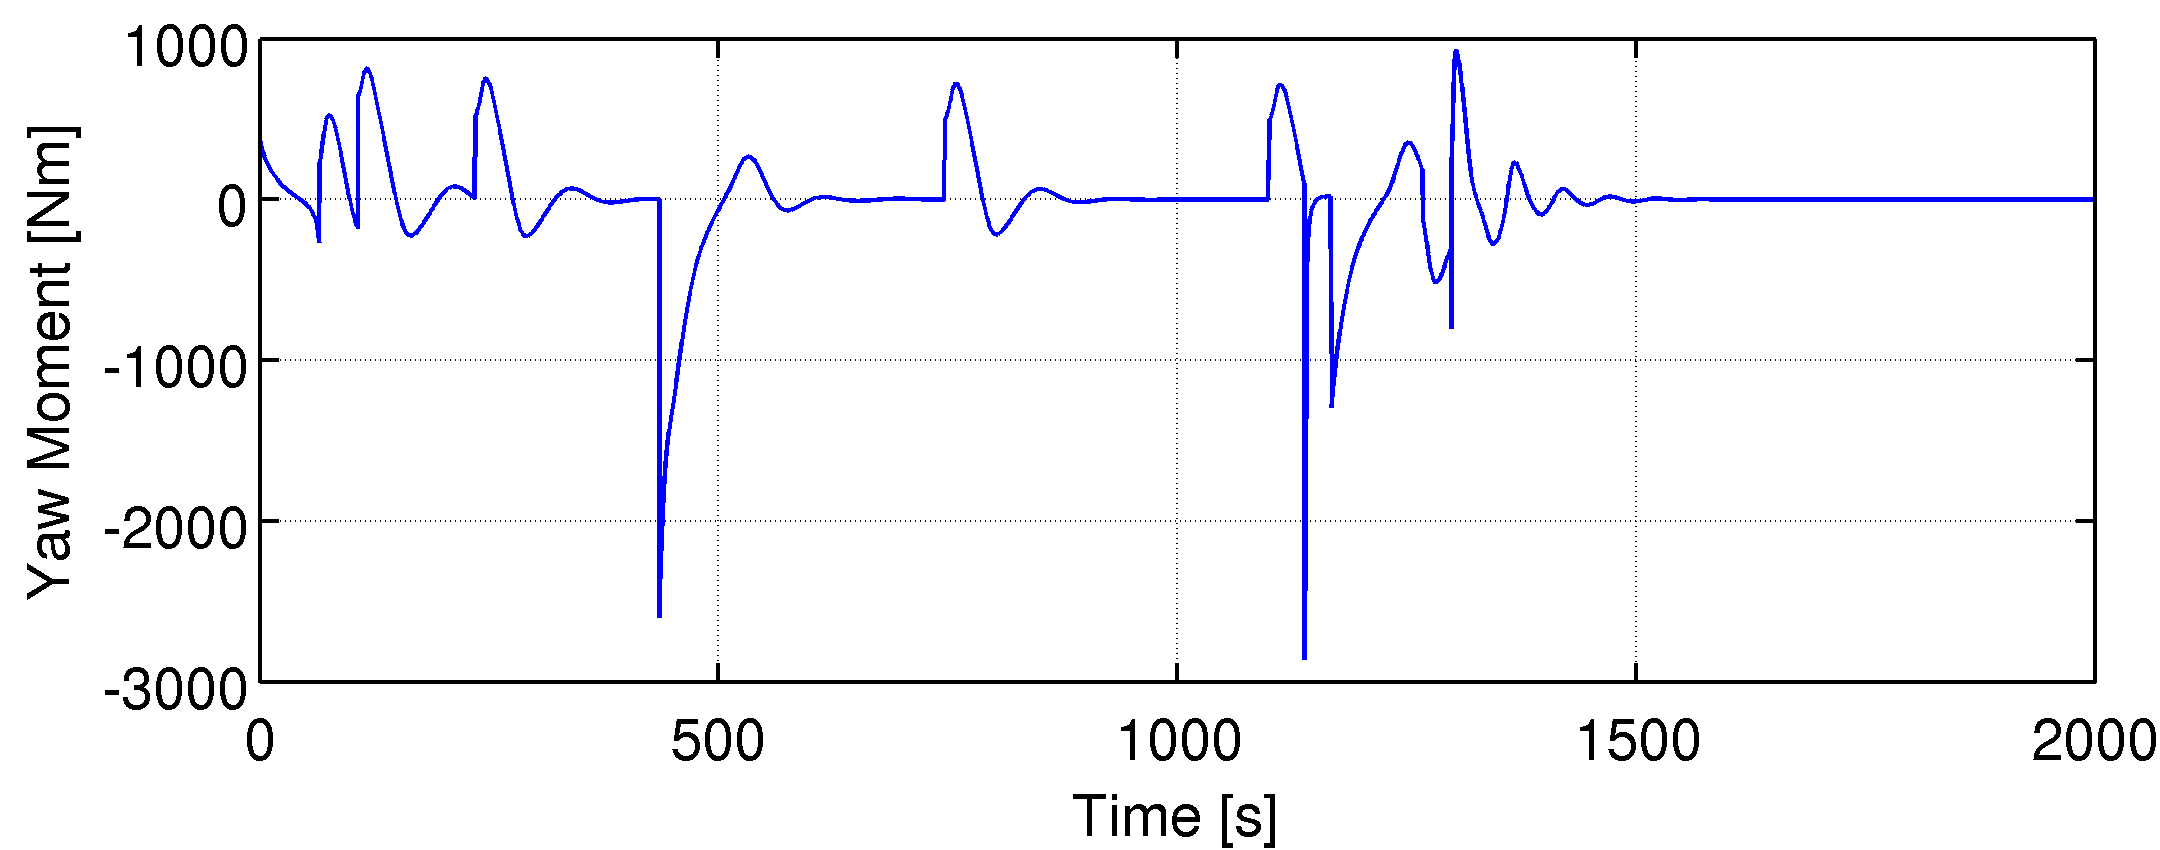
\includegraphics[width=0.7\textwidth]{pics/ch4_yawmoment}}
		\caption{Plots describing the close relation of yaw moment and roll angle}
		\label{fig:ch4_rollyawmoment}
	\end{figure}
	Figure~\ref{fig:ch4_rollyawmoment} shows the relation between commanded yaw moment and the roll angle.
	Clearly there are coupling effects which causes the roll angle to change a few degrees. The roll angle
	magnitude are about $2^\circ$ when the \textit{surge}-velocity are 2 m/s. But the roll angle are not
	of greate concern when carrying out this kind of inspection missions, as these simulations show.

	
	The main propeller gives a moment in roll. This moment are disregarded in the simulations, but might
	become important. The main propeller are described by the followin relations
	\begin{equation}
		\begin{aligned}
			\tau_1 &= T_{nn} n^2 + T_{un} n u \\
			\tau_4 &= Q_{nn} n^2 + Q_{un} n u
		\end{aligned}
	\end{equation}
	where $n$ are the angular speed of the main propeller in Revolutions per minute, and $u$ are again the
	surge velocity. The second terms in the equation above are terms descibing loss-of-force due to
	forward speed. The moment in roll are actually countered by weightin the AUV down on one side so that when
	the it reaches cruice velocity the AUV have zero roll angle. \cite{Bjorn_gjelstad_talk}

	This is due to some of the design features of \textit{HUGIN} AUV. It is designed to be
	asymptotically stable in roll, due to the centre of bouyancy (CB) are located not exactly in the centre of
	gravity (CG). The AUV would not need roll stabilisation becuase it shows to be very stable in roll.
	Another case is that if roll stabilisation were to be implemented it would be done by using the
	rudders, and this would cause an increase in power consumption that would not be advisable. 


\section{Energy Consumption}
	The energy consumption of an AUV are of extreme importance. When a customer are buying this type of
	vessel one of the criteria are operation time. For an AUV which are untethered and have limited power 
	supply the operation time might vary greatly due to installed sensors and operating conditions.

	The standard sensor suite on the \hugin AUV are a Side Scan Sonar, Doppler Velocity Log, Depth meter,
	Multibeam Echosounder, and the INS navigation system. The operation time would be around 10-20 houres,
	dependent on velocity and sensor use. The main objective of the guidance system after the inpsection
	part is to maximise the operating time. This can be done in numerous ways, and should be a part of the
	design procedure when designing the guidance system for the real thing.

	The actuator set-up of \hugin  are with 4 rudders, one main propeller and 4 thurusters. This renders
	the AUV controllable in 5 DOFs. The thrusters demand more power than the main propeller
	and rudders, and have been completely disregarded throughout this report. The most energy efficient
	way of moving is using the main propeller and the rudders to navigate the AUV.

	The most energy efficient way of guiding an AUV is to use its main propeller and rudders. But there
	might be different ways of optimising the power consumption with regard to how the AUV are searching
	for and tracking the pipeline. The forces produced by for instance the vertical rudders, the moment
	produced by this rudders are proportional to the surge velocity squared.
		\begin{equation}
			\tau_6 = Y_{u\psi} \delta u^2
		\end{equation}
	where $\delta$ are the angle of the rudder, and $Y_{u \psi}$ are some constant describing the rudder
	areal. This means that the effect of the rudders are greatly dependent on the forward speed. This is
	not taken into account in the designed controller and have to be compensated in a more advanced
	controller, or it can be taken care of in the control allocation problem not considered in this
	report.  

	The energy consumption are very dependent on how the AUV moves. If it are taking unnescecary turns the
	movemente pattern are not optimal. In this sense the shortest distance traveled is the most optimal
	movement pattern. The guidance system should always take the shortes path to the goal, if the
	environment allows it. 
	
	\cite{fuel_optimal_control} proposes an optimal guidance scheme. Using the
	fuel consumption as a performance index and optimize with regard to the current forces in the area of
	interest. It requiers knowledge of the currents in the area \'a priori and utilizes this to calculate
	the otimal trajectory from one point to the next. This gives good theoretical results but the downside
	is that knowledge about the current forces in an area are rarely konwn, and if they are known they are
	probably not very exact. But this scheme might help to save energy, but are only aplicable to a
	pipeline inspection mission when the AUV are moving to or from the pipeline, not when tracking or
	searching.
	
	Either way, it is important to chose the right way to go when you have limited power capability. This
	motivates the use of more sensors, to increase the chances of not giving bad and erronous sensor data
	to the guidance system. The guidance system needs to be robust and take the right descision. Too
	maximise the operation time it can not afford to take wrong decisions. This is almost impossible to
	achieve and can only be done through extencive testing of the complete syste, it is important tto
	chose the right way to go when you have limited power capability.This motivates the use of more
	sensors, to increase the chances of not giving bad and erronous sensor data to the guidance system.
	IThe guidance system needs to be robust and take the right descisio. Too maximise the operation time
	it can not afford to take wrong decisions. This is almost impossible to achieve and mcan only be done
	through extencive testing of the complete system.

\section{Optimal Search Pattern}
	As discussed above, the need for efficient search pattern are crucial to maximising the operation
	time. Search patterns might vary form case to case. The search patten should be dependent on how well
	the mission area are known and how sure one can be about the \'a priori data about the pipeline
	condition, sea bottom obstacles and features. Are there obstacles in the area which might be used for
	position identification and navigation. Or are there obstacles in the area that the AUV should avoid
	completely, such as mines. 

\section{How valid are the results?}
	The analysis done in this report are ment to be a pre-study of the problems assosiated with this
	complex pipeline inspection problem.

